%!TEX root = ../main_article.tex

\section{Introduction}
\label{section:1}

Code search plays a vital role in the software development process, which is an essential field of Software Engineering and studies the semantic similarity between natural language queries and program code. Recent years have witnessed a massive increment in source code. The statistic shows that more than 60 million new projects were created only in 2020 (\citealp{abs-2110-10246}). Thus, code search engines can improve the development efficiency of program developers, enabling them to search for existing code or examples of some API (Application Programming Interface) instead of “rebuilding wheels.” 

As deep learning has grown by leaps and bounds in recent years, a number of methods have been proposed in code search, such as Recurrent Neural Network (RNN) based models (\citealp{DeepCS}), CNNs (Convolutional Neural Networks) based models (\citealp{CQIL, ShuaiX0Y0L20}), graph based models (\citealp{, GuCM21}), and Pre-trained Language Models (PLMs) based models (\citealp{CodeBERT,CoCLR,GraphCodeBERT,UniXcoder}). 

From the view of PLMs, all of them have well performance in code search, with complex model architecture and advanced training techniques. However, PLMs often treat code search as a downstream task, which means researchers can pre-train a model with hybrid objectives and multiple program language code data, then fine-tune it in a specific program language for code search (\citealp{UniXcoder,CodeBERT,GraphCodeBERT,SPTCode}). Our empirical study shows that there might be a performance decline when fine-tuning with data in multiple languages. Table~\ref{tab:comparison} shows MRR (Mean Reciprocal Rank, \citealp{MRR}) comparisons between single program language fine-tuned models, and multiple program language fine-tuned models. The left first column indicates what program languages have been used in fine-tuning and the rest columns show the search performance toward a specific language according to the first column. Similar to multilingual models (\citealp{multilingualModel,YangYCD21}), code information can be roughly divided into identity information, distinguishing code from another code written in different program languages, and semantic information, which reveals its intention and with a corresponding natural language description. In code search, code semantic information is only needed, for it is matched with specific queries. The identity information may confound model training and decrease performance when fine-tuning with multiple program language data. We view identity information as the signal that helps to distinguish different program language data, which has the same idea as classification. Semantic information reveals the code intention, which is related to code search.
% \begin{figure}[htb]
% 	\centering
% 	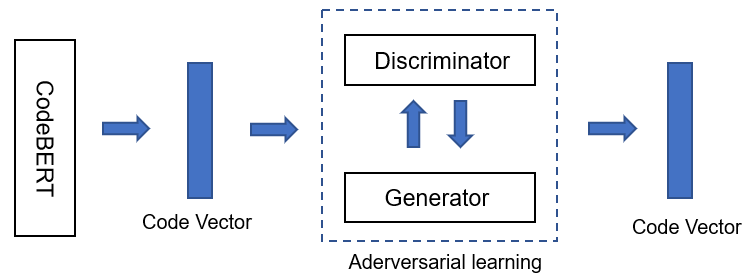
\includegraphics[width=1\linewidth]{imgs/structure.png}
% 	% \vspace{-15pt}
% 	\caption{Structure of the search enhancement framework.}
% 	% \vspace{-12pt}
% 	\label{fig:structure}
% \end{figure}

Therefore, we want to reduce the identity information of the embedding vector given by code search pre-trained models. We propose two strategies for disentangling.  The first is to follow the idea of GAN (Generative Adversarial Network, \citealp{goodfellow2020generative}) and leverage a generator to generate identity free embedding vectors. The second is to use an additional network to obtain identity and semantic vectors separately. We consider maximizing KL divergence in the loss function.

In summary, our contributions are:
\begin{enumerate} 
\item Reveal the performance decline problem that appears when fine-tuning code search with multiple program languages.
\item We propose different disentangling strategies for splitting identity and semantic information of the embedding vectors output by pre-train code models.
\end{enumerate}


% Table generated by Excel2LaTeX from sheet 'Sheet1'
\begin{table}[htbp]
	\centering
	\caption{Performance comparisons with different fine-tuning program languages}
	\vspace{-5pt}
	\resizebox{\linewidth}{!}{
	\begin{tabular}{lrrrr}
		\toprule
        & Python & Go  & Java & PHP \\
    \midrule
    Python & 0.369 & \_  & \_  &  \\
    Go  & \_  & 0.904 & \_  & \_ \\
    Java & \_  & \_  & 0.764 & \_ \\
    PHP & \_  & \_  & \_  & 0.708 \\
    Python\_Java & 0.468 & \_  & 0.708 $\downarrow$ & \_ \\
    Python\_Go & 0.404 & 0.882 $\downarrow$ & \_  & \_ \\
    Java\_Go & \_  & 0.902 $\downarrow$ & 0.724 $\downarrow$ & \_ \\
    Java\_PHP & \_  & \_  & 0.743 $\downarrow$ & 0.707 $\downarrow$ \\
    Java\_Python\_Go & 0.571 & 0.889 $\downarrow$ & 0.701 $\downarrow$ & \_ \\
    \bottomrule
	\end{tabular}%
	}
	\label{tab:comparison}%
	\vspace{-10	pt}
\end{table}%
